\chapter{Results}
\label{ch:results}

The results of the experiments conducted in this study are presented in this chapter. The findings are organized according to the research questions outlined in Chapter \ref{ch:intro}. Each section provides a detailed analysis of the results, including relevant figures and tables to support the findings. Detailed analysis of the results will follow in Chapter \ref{ch:discuss}.

\section{Manual Exploration of Dataset}

\begin{figure}[h]
    \centering
    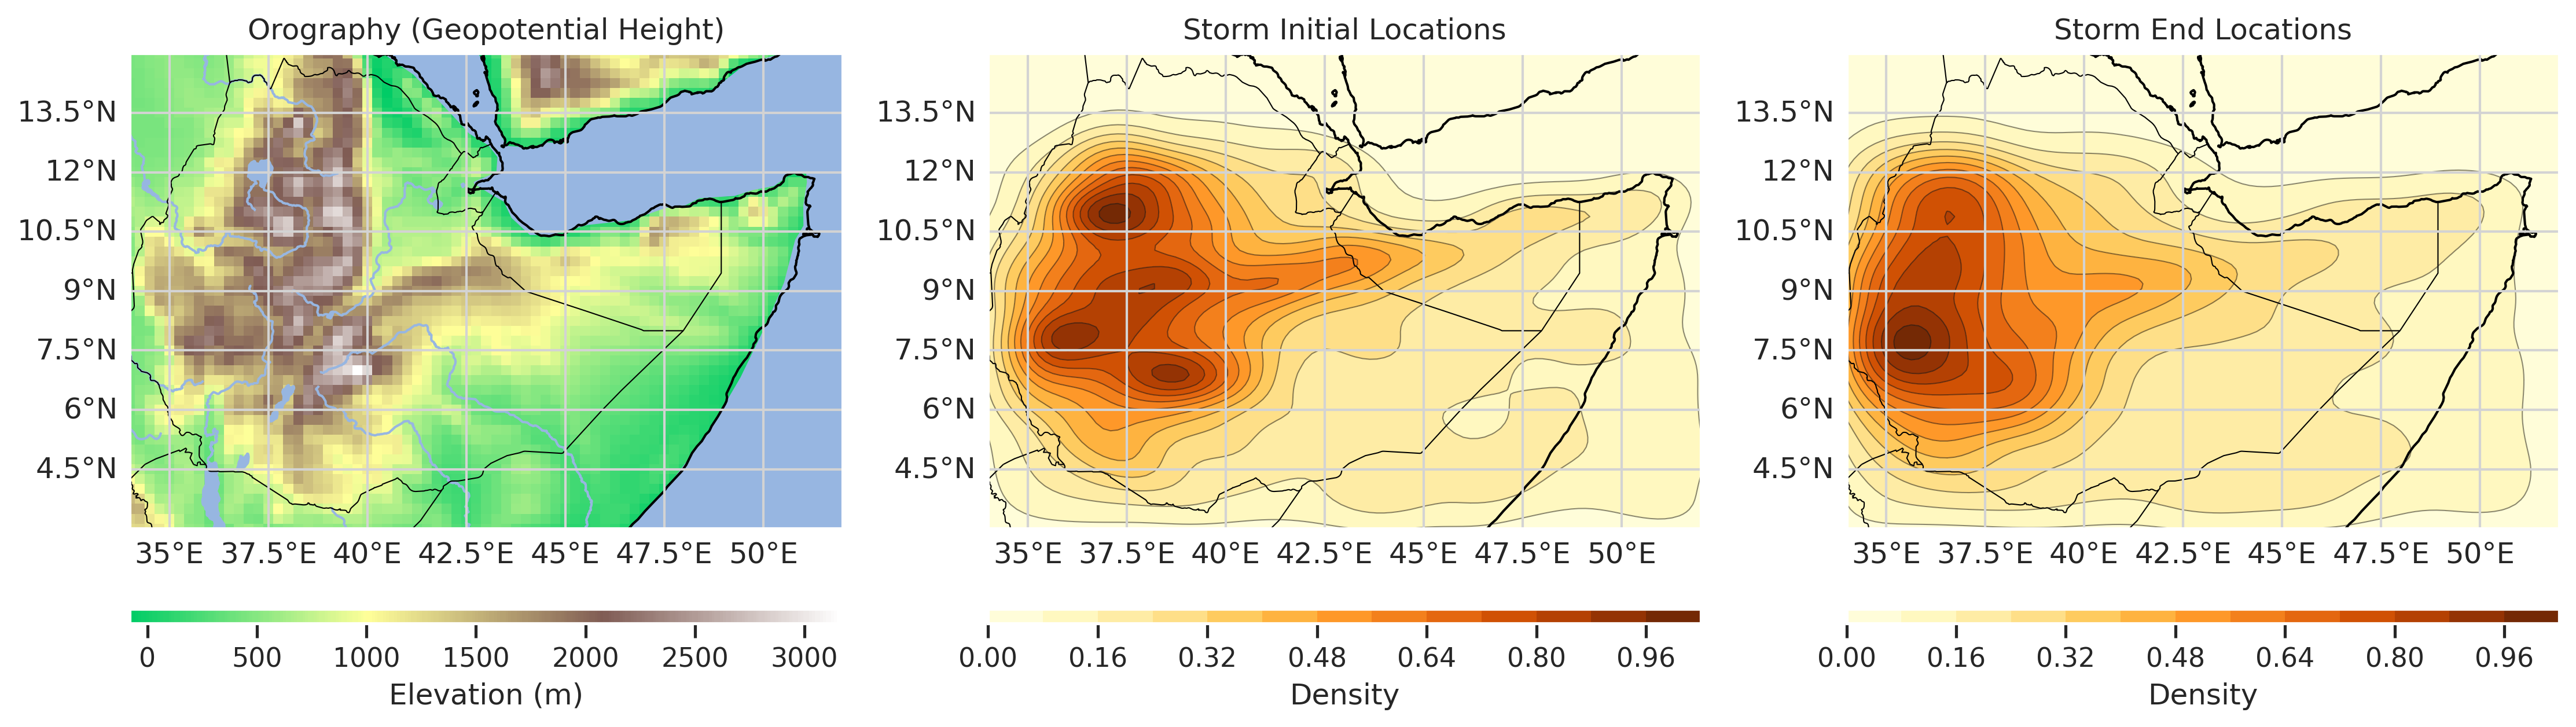
\includegraphics[width=\textwidth]{../figures/generated/orography_storm_init_end_kde.png}
    \caption{Storm First and Last Observation by Location.}
    \label{fig:orography_storm_init_end_kde}
\end{figure}

\begin{figure}[h]
    \centering
    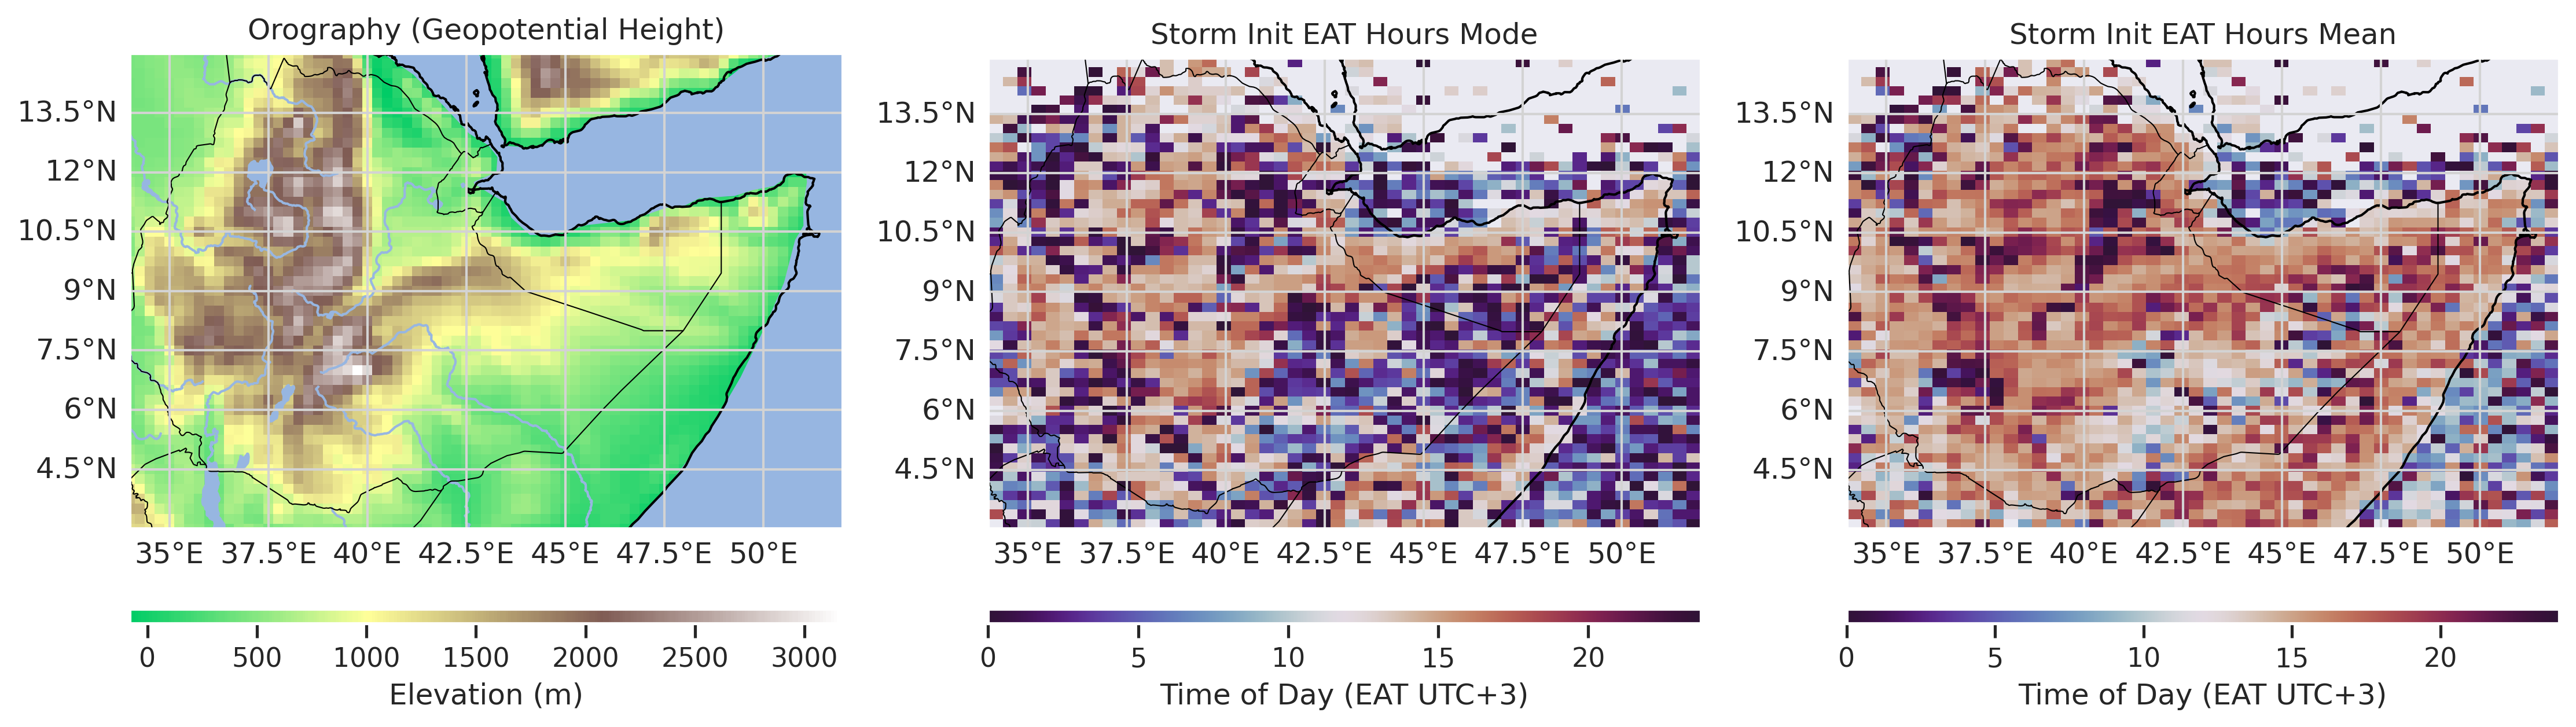
\includegraphics[width=\textwidth]{../figures/generated/orography_storm_init_eat_hours_mode_mean.png}
    \caption{Storm Genesis Local Time by Location.}
    \label{fig:orography_storm_init_eat_hours_mode_mean}
\end{figure}

\section{Experimental Setup}

For all experiments listed below, two models were trained: once using all available features and once using only ERA5 meteorological features. This approach allows for a comparison of model performance when utilising only focused subset of meteorological variables. While it is clear from the manual exploration above that storm location and orography will play a major role, it's possible that those features could confound the effects of other environmental factors like soil moisture or skin temperature. Thus, through this setup, we ensure that one model is exclusively learning from the meteorology. If model performance differs significantly, this would imply that the geographic, topological, or temporal features contain unique information not captured by the meteorological features. Through a comparison of relative feature importance of the meteorological features, we can also gain insights into their interaction with the other features. In addition, for the storm aggregate prediction tasks, two additional models were trained using only the first observation of each storm, again comparing all features versus only ERA5 features. This aspect of the setup aims to evaluate the predictive power of initial storm observations.

\section{Predict Storm Aggregate Features}

These experiments aim to predict the overall characteristics of a storm based on its initial observation.

\subsection{Storm Max Intensity}

\subsubsection{All Observations}

\begin{figure}[h]
    \centering
    \missingfigure{2x2 Subplots: Row 1: Actual vs Predicted scatter with regression, Row 2: SHAP beeswarm top features.}
    \caption{Comparison of performance and top features for storm max intensity.}
    \label{fig:storm_max_intensity_summary}
\end{figure}

\subsubsection{First Points Only}

\begin{figure}[h]
    \centering
    \missingfigure{2x2 Subplots: Row 1: Actual vs Predicted scatter with regression, Row 2: SHAP beeswarm top features.}
    \caption{Comparison of performance and top features for storm max intensity (First Points Only).}
    \label{fig:storm_max_intensity_first_points_summary}
\end{figure}

\subsection{Storm Direction}

\subsubsection{All Observations}

\begin{figure}[h]
    \centering
    \missingfigure{2x2 Subplots: Row 1: Actual vs Predicted scatter with regression, Row 2: SHAP beeswarm top features.}
    \caption{Comparison of performance and top features for storm direction.}
    \label{fig:storm_direction_summary}
\end{figure}

\subsubsection{First Points Only}

\begin{figure}[h]
    \centering
    \missingfigure{2x2 Subplots: Row 1: Actual vs Predicted scatter with regression, Row 2: SHAP beeswarm top features.}
    \caption{Comparison of performance and top features for storm direction (First Points Only).}
    \label{fig:storm_direction_first_points_summary}
\end{figure}

\subsection{Predict Immediate Characteristics at an Observation}

These experiments aim to predict the immediate characteristics of a storm based on its current observation.

\subsection{Intensification}

\begin{figure}[h]
    \centering
    \missingfigure{2x2 Subplots: Row 1: Actual vs Predicted scatter with regression, Row 2: SHAP beeswarm top features.}
    \caption{Comparison of performance and top features for intensification.}
    \label{fig:obs_intensification_summary}
\end{figure}

\subsection{Direction}

\begin{figure}[h]
    \centering
    \missingfigure{2x2 Subplots: Row 1: Actual vs Predicted scatter with regression, Row 2: SHAP beeswarm top features.}
    \caption{Comparison of performance and top features for direction.}
    \label{fig:obs_direction_summary}
\end{figure}

\subsection{Distance}

\begin{figure}[h]
    \centering
    \missingfigure{2x2 Subplots: Row 1: Actual vs Predicted scatter with regression, Row 2: SHAP beeswarm top features.}
    \caption{Comparison of performance and top features for distance.}
    \label{fig:obs_distance_summary}
\end{figure}

\subsection{Precipitation}

\begin{figure}[h]
    \centering
    \missingfigure{2x2 Subplots: Row 1: Actual vs Predicted scatter with regression, Row 2: SHAP beeswarm top features.}
    \caption{Comparison of performance and top features for precipitation.}
    \label{fig:obs_precipitation_summary}
\end{figure}